
%% bare_conf.tex
%% V1.3
%% 2007/01/11
%% by Michael Shell
%% See:
%% http://www.michaelshell.org/
%% for current contact information.
%%
%% This is a skeleton file demonstrating the use of IEEEtran.cls
%% (requires IEEEtran.cls version 1.7 or later) with an IEEE conference paper.
%%
%% Support sites:
%% http://www.michaelshell.org/tex/ieeetran/
%% http://www.ctan.org/tex-archive/macros/latex/contrib/IEEEtran/
%% and
%% http://www.ieee.org/

%%*************************************************************************
%% Legal Notice:
%% This code is offered as-is without any warranty either expressed or
%% implied; without even the implied warranty of MERCHANTABILITY or
%% FITNESS FOR A PARTICULAR PURPOSE!
%% User assumes all risk.
%% In no event shall IEEE or any contributor to this code be liable for
%% any damages or losses, including, but not limited to, incidental,
%% consequential, or any other damages, resulting from the use or misuse
%% of any information contained here.
%%
%% All comments are the opinions of their respective authors and are not
%% necessarily endorsed by the IEEE.
%%
%% This work is distributed under the LaTeX Project Public License (LPPL)
%% ( http://www.latex-project.org/ ) version 1.3, and may be freely used,
%% distributed and modified. A copy of the LPPL, version 1.3, is included
%% in the base LaTeX documentation of all distributions of LaTeX released
%% 2003/12/01 or later.
%% Retain all contribution notices and credits.
%% ** Modified files should be clearly indicated as such, including  **
%% ** renaming them and changing author support contact information. **
%%
%% File list of work: IEEEtran.cls, IEEEtran_HOWTO.pdf, bare_adv.tex,
%%                    bare_conf.tex, bare_jrnl.tex, bare_jrnl_compsoc.tex
%%*************************************************************************

% *** Authors should verify (and, if needed, correct) their LaTeX system  ***
% *** with the testflow diagnostic prior to trusting their LaTeX platform ***
% *** with production work. IEEE's font choices can trigger bugs that do  ***
% *** not appear when using other class files.                            ***
% The testflow support page is at:
% http://www.michaelshell.org/tex/testflow/



% Note that the a4paper option is mainly intended so that authors in
% countries using A4 can easily print to A4 and see how their papers will
% look in print - the typesetting of the document will not typically be
% affected with changes in paper size (but the bottom and side margins will).
% Use the testflow package mentioned above to verify correct handling of
% both paper sizes by the user's LaTeX system.
%
% Also note that the "draftcls" or "draftclsnofoot", not "draft", option
% should be used if it is desired that the figures are to be displayed in
% draft mode.
%
\documentclass[conference]{IEEEtran}
% Add the compsoc option for Computer Society conferences.
%
% If IEEEtran.cls has not been installed into the LaTeX system files,
% manually specify the path to it like:
% \documentclass[conference]{../sty/IEEEtran}





% Some very useful LaTeX packages include:
% (uncomment the ones you want to load)


% *** MISC UTILITY PACKAGES ***
%
%\usepackage{ifpdf}
% Heiko Oberdiek's ifpdf.sty is very useful if you need conditional
% compilation based on whether the output is pdf or dvi.
% usage:
% \ifpdf
%   % pdf code
% \else
%   % dvi code
% \fi
% The latest version of ifpdf.sty can be obtained from:
% http://www.ctan.org/tex-archive/macros/latex/contrib/oberdiek/
% Also, note that IEEEtran.cls V1.7 and later provides a builtin
% \ifCLASSINFOpdf conditional that works the same way.
% When switching from latex to pdflatex and vice-versa, the compiler may
% have to be run twice to clear warning/error messages.






% *** CITATION PACKAGES ***
%
%\usepackage{cite}
% cite.sty was written by Donald Arseneau
% V1.6 and later of IEEEtran pre-defines the format of the cite.sty package
% \cite{} output to follow that of IEEE. Loading the cite package will
% result in citation numbers being automatically sorted and properly
% "compressed/ranged". e.g., [1], [9], [2], [7], [5], [6] without using
% cite.sty will become [1], [2], [5]--[7], [9] using cite.sty. cite.sty's
% \cite will automatically add leading space, if needed. Use cite.sty's
% noadjust option (cite.sty V3.8 and later) if you want to turn this off.
% cite.sty is already installed on most LaTeX systems. Be sure and use
% version 4.0 (2003-05-27) and later if using hyperref.sty. cite.sty does
% not currently provide for hyperlinked citations.
% The latest version can be obtained at:
% http://www.ctan.org/tex-archive/macros/latex/contrib/cite/
% The documentation is contained in the cite.sty file itself.






% *** GRAPHICS RELATED PACKAGES ***
%
\ifCLASSINFOpdf
  % \usepackage[pdftex]{graphicx}
  % declare the path(s) where your graphic files are
  % \graphicspath{{../pdf/}{../jpeg/}}
  % and their extensions so you won't have to specify these with
  % every instance of \includegraphics
  % \DeclareGraphicsExtensions{.pdf,.jpeg,.png}
\else
  % or other class option (dvipsone, dvipdf, if not using dvips). graphicx
  % will default to the driver specified in the system graphics.cfg if no
  % driver is specified.
  % \usepackage[dvips]{graphicx}
  % declare the path(s) where your graphic files are
  % \graphicspath{{../eps/}}
  % and their extensions so you won't have to specify these with
  % every instance of \includegraphics
  % \DeclareGraphicsExtensions{.eps}
\fi
% graphicx was written by David Carlisle and Sebastian Rahtz. It is
% required if you want graphics, photos, etc. graphicx.sty is already
% installed on most LaTeX systems. The latest version and documentation can
% be obtained at:
% http://www.ctan.org/tex-archive/macros/latex/required/graphics/
% Another good source of documentation is "Using Imported Graphics in
% LaTeX2e" by Keith Reckdahl which can be found as epslatex.ps or
% epslatex.pdf at: http://www.ctan.org/tex-archive/info/
%
% latex, and pdflatex in dvi mode, support graphics in encapsulated
% postscript (.eps) format. pdflatex in pdf mode supports graphics
% in .pdf, .jpeg, .png and .mps (metapost) formats. Users should ensure
% that all non-photo figures use a vector format (.eps, .pdf, .mps) and
% not a bitmapped formats (.jpeg, .png). IEEE frowns on bitmapped formats
% which can result in "jaggedy"/blurry rendering of lines and letters as
% well as large increases in file sizes.
%
% You can find documentation about the pdfTeX application at:
% http://www.tug.org/applications/pdftex





% *** MATH PACKAGES ***
%
%\usepackage[cmex10]{amsmath}
% A popular package from the American Mathematical Society that provides
% many useful and powerful commands for dealing with mathematics. If using
% it, be sure to load this package with the cmex10 option to ensure that
% only type 1 fonts will utilized at all point sizes. Without this option,
% it is possible that some math symbols, particularly those within
% footnotes, will be rendered in bitmap form which will result in a
% document that can not be IEEE Xplore compliant!
%
% Also, note that the amsmath package sets \interdisplaylinepenalty to 10000
% thus preventing page breaks from occurring within multiline equations. Use:
%\interdisplaylinepenalty=2500
% after loading amsmath to restore such page breaks as IEEEtran.cls normally
% does. amsmath.sty is already installed on most LaTeX systems. The latest
% version and documentation can be obtained at:
% http://www.ctan.org/tex-archive/macros/latex/required/amslatex/math/





% *** SPECIALIZED LIST PACKAGES ***
%
%\usepackage{algorithmic}
% algorithmic.sty was written by Peter Williams and Rogerio Brito.
% This package provides an algorithmic environment fo describing algorithms.
% You can use the algorithmic environment in-text or within a figure
% environment to provide for a floating algorithm. Do NOT use the algorithm
% floating environment provided by algorithm.sty (by the same authors) or
% algorithm2e.sty (by Christophe Fiorio) as IEEE does not use dedicated
% algorithm float types and packages that provide these will not provide
% correct IEEE style captions. The latest version and documentation of
% algorithmic.sty can be obtained at:
% http://www.ctan.org/tex-archive/macros/latex/contrib/algorithms/
% There is also a support site at:
% http://algorithms.berlios.de/index.html
% Also of interest may be the (relatively newer and more customizable)
% algorithmicx.sty package by Szasz Janos:
% http://www.ctan.org/tex-archive/macros/latex/contrib/algorithmicx/




% *** ALIGNMENT PACKAGES ***
%
%\usepackage{array}
% Frank Mittelbach's and David Carlisle's array.sty patches and improves
% the standard LaTeX2e array and tabular environments to provide better
% appearance and additional user controls. As the default LaTeX2e table
% generation code is lacking to the point of almost being broken with
% respect to the quality of the end results, all users are strongly
% advised to use an enhanced (at the very least that provided by array.sty)
% set of table tools. array.sty is already installed on most systems. The
% latest version and documentation can be obtained at:
% http://www.ctan.org/tex-archive/macros/latex/required/tools/


%\usepackage{mdwmath}
%\usepackage{mdwtab}
% Also highly recommended is Mark Wooding's extremely powerful MDW tools,
% especially mdwmath.sty and mdwtab.sty which are used to format equations
% and tables, respectively. The MDWtools set is already installed on most
% LaTeX systems. The lastest version and documentation is available at:
% http://www.ctan.org/tex-archive/macros/latex/contrib/mdwtools/


% IEEEtran contains the IEEEeqnarray family of commands that can be used to
% generate multiline equations as well as matrices, tables, etc., of high
% quality.


%\usepackage{eqparbox}
% Also of notable interest is Scott Pakin's eqparbox package for creating
% (automatically sized) equal width boxes - aka "natural width parboxes".
% Available at:
% http://www.ctan.org/tex-archive/macros/latex/contrib/eqparbox/





% *** SUBFIGURE PACKAGES ***
%\usepackage[tight,footnotesize]{subfigure}
% subfigure.sty was written by Steven Douglas Cochran. This package makes it
% easy to put subfigures in your figures. e.g., "Figure 1a and 1b". For IEEE
% work, it is a good idea to load it with the tight package option to reduce
% the amount of white space around the subfigures. subfigure.sty is already
% installed on most LaTeX systems. The latest version and documentation can
% be obtained at:
% http://www.ctan.org/tex-archive/obsolete/macros/latex/contrib/subfigure/
% subfigure.sty has been superceeded by subfig.sty.



%\usepackage[caption=false]{caption}
%\usepackage[font=footnotesize]{subfig}
% subfig.sty, also written by Steven Douglas Cochran, is the modern
% replacement for subfigure.sty. However, subfig.sty requires and
% automatically loads Axel Sommerfeldt's caption.sty which will override
% IEEEtran.cls handling of captions and this will result in nonIEEE style
% figure/table captions. To prevent this problem, be sure and preload
% caption.sty with its "caption=false" package option. This is will preserve
% IEEEtran.cls handing of captions. Version 1.3 (2005/06/28) and later
% (recommended due to many improvements over 1.2) of subfig.sty supports
% the caption=false option directly:
%\usepackage[caption=false,font=footnotesize]{subfig}
%
% The latest version and documentation can be obtained at:
% http://www.ctan.org/tex-archive/macros/latex/contrib/subfig/
% The latest version and documentation of caption.sty can be obtained at:
% http://www.ctan.org/tex-archive/macros/latex/contrib/caption/




% *** FLOAT PACKAGES ***
%
%\usepackage{fixltx2e}
% fixltx2e, the successor to the earlier fix2col.sty, was written by
% Frank Mittelbach and David Carlisle. This package corrects a few problems
% in the LaTeX2e kernel, the most notable of which is that in current
% LaTeX2e releases, the ordering of single and double column floats is not
% guaranteed to be preserved. Thus, an unpatched LaTeX2e can allow a
% single column figure to be placed prior to an earlier double column
% figure. The latest version and documentation can be found at:
% http://www.ctan.org/tex-archive/macros/latex/base/



%\usepackage{stfloats}
% stfloats.sty was written by Sigitas Tolusis. This package gives LaTeX2e
% the ability to do double column floats at the bottom of the page as well
% as the top. (e.g., "\begin{figure*}[!b]" is not normally possible in
% LaTeX2e). It also provides a command:
%\fnbelowfloat
% to enable the placement of footnotes below bottom floats (the standard
% LaTeX2e kernel puts them above bottom floats). This is an invasive package
% which rewrites many portions of the LaTeX2e float routines. It may not work
% with other packages that modify the LaTeX2e float routines. The latest
% version and documentation can be obtained at:
% http://www.ctan.org/tex-archive/macros/latex/contrib/sttools/
% Documentation is contained in the stfloats.sty comments as well as in the
% presfull.pdf file. Do not use the stfloats baselinefloat ability as IEEE
% does not allow \baselineskip to stretch. Authors submitting work to the
% IEEE should note that IEEE rarely uses double column equations and
% that authors should try to avoid such use. Do not be tempted to use the
% cuted.sty or midfloat.sty packages (also by Sigitas Tolusis) as IEEE does
% not format its papers in such ways.





% *** PDF, URL AND HYPERLINK PACKAGES ***
%
%\usepackage{url}
% url.sty was written by Donald Arseneau. It provides better support for
% handling and breaking URLs. url.sty is already installed on most LaTeX
% systems. The latest version can be obtained at:
% http://www.ctan.org/tex-archive/macros/latex/contrib/misc/
% Read the url.sty source comments for usage information. Basically,
% \url{my_url_here}.





% *** Do not adjust lengths that control margins, column widths, etc. ***
% *** Do not use packages that alter fonts (such as pslatex).         ***
% There should be no need to do such things with IEEEtran.cls V1.6 and later.
% (Unless specifically asked to do so by the journal or conference you plan
% to submit to, of course. )

\usepackage[linesnumbered,ruled]{algorithm2e}
%\usepackage[pdftex]{graphicx}
% For figures
\usepackage{graphicx} % more modern
\usepackage{epsfig} % less modern
\usepackage{subfigure}
\usepackage{enumerate}
\usepackage{amssymb}
%\usepackage[pdftex]{graphicx}
% For figures
\usepackage{graphicx} % more modern
%\usepackage{epsfig} % less modern
\usepackage{subfigure}

\usepackage{mathrsfs}
\usepackage{amsmath}  
% Package to generate and customize Algorithm as per ACM style
\usepackage[ruled]{algorithm2e}
\usepackage{color}
%\DeclareCaptionType{copyrightbox}
%\usepackage{amsthm}
\newtheorem{myprop}{Proposition}

% correct bad hyphenation here
\hyphenation{op-tical net-works semi-conduc-tor}


\begin{document}
%
% paper title
% can use linebreaks \\ within to get better formatting as desired
\title{Multi-view Failure Analysis on 
Multivariate Time-series Data
}

\author{
\IEEEauthorblockN{
Hao Huang\IEEEauthorrefmark{1},
Yunwen Xu\IEEEauthorrefmark{2}
and Shinjae Yoo\IEEEauthorrefmark{3}
}
\IEEEauthorblockA{\IEEEauthorrefmark{1}Machine Learning Lab, GE Global Research, Email: haohuangcssbu@gmail.com}
\IEEEauthorblockA{\IEEEauthorrefmark{2}Core Machine Learning Team, Amazon, Email: xuyunwen04@gmail.com}
\IEEEauthorblockA{\IEEEauthorrefmark{3}Computational Science Center, Brookhaven National Lab, Email: sjyoo@bnl.gov}
}
% make the title area
\maketitle

\begin{abstract}
 to be finished
%\boldmath
%Spectral Embedding is one of the most effective dimension reduction algorithms in data mining. However, its computation complexity has to be mitigated in order to apply it for real-world large scale data analysis. Many researches have been focusing on developing approximate spectral embeddings which are more efficient, but meanwhile far less effective. This paper proposes Diverse Power Iteration Embeddings (DPIE), which not only retains the similar efficiency of power iteration methods but also produces a series of diverse and more effective embedding vectors. We test this novel method by applying it to various data mining applications (e.g. clustering, anomaly detection and feature selection) and evaluating their performance improvements. The experimental results show our proposed DPIE is more effective than popular spectral approximation methods, and obtains the similar quality of classic spectral embedding derived from eigen-decompositions. Moreover it is extremely fast on big data applications. For example in terms of clustering result, DPIE achieves as good as $95\%$ of classic spectral clustering on the complex datasets but $4000+$ times faster in limited memory environment.
\end{abstract}

\IEEEpeerreviewmaketitle

\section{Introduction}
\label{sec:MAMT:intro}

With the rapid advances in sensor design, data storage and networking, we are facing an explosive growth of complexity in analyzing failure (or event) in multivariate time series data. Failure analytics system can be identified from the knowledge data discovery process where the output gives the fault signatures that relate to the failure, while the input data correspond to recorded sensor measurements that are considered as features. These high-frequent, large-scale data often require fleet level analysis, which not only involve the event assets, but also the healthy assets (usually much more than those event ones), therefore a unique fault signature relates to the failure can be found and a detector with low-false-alarm-rate can be created. The output of such signature should consist of or directly relate to the weighting of input sensor, therefore more effectively support the root cause analysis. Furthermore, a forecast model can be built consequently that gives early warning of the same failure in the future.      


Besides large-volume of data on the fleet level, we are also facing the following challenges in finding such signatures: 
1) The fault signatures usually exist in multivariate time series involving a lot of assets, which makes it hard to detect by any univariate and uni-asset analytics;
2) While the event time can be known, the time that faulty signatures happen is usually unknown, and could be different from case to case, which makes it difficult to detect by any (semi-)supervised machine learning techniques. 

Figure~\ref{fig:MAMT:motivation} shows the two signature examples from ground truth by domain experts. In Figure~\ref{fig:MAMT:motivation:01} the signature appears $15$ days before the failure, and the signature is with small value on feature A and large value on feature B. While in Figure~\ref{fig:MAMT:motivation:02} the signature appears almost one month before the failure, where there is a level-shift on feature C that can be depicted by auto-correlation (auc). It is interesting and important to notice that 1) both of these examples show significant lag between signature and failure, and 2) the lasting time of signature are different which is also unknown for the analytics. As a matter of fact, this ``lag" patterns are usual and could be with different reasons. One of the reasons is that the input sensors could be indirectly related to the failure. For example, an engine stall event may happen because some component is crack. But due to the complexity of the engine design, it takes certain time for such fault propagate to the whole system which leads to the final failure. Right before the crack, the vibration sensors of the faulty component can show strong vibrating patterns, which can be viewed as the faulty signature. But once the crack happen, this component becomes unconnected to the whole system and the vibration sensor recording become stable. Therefore the signature cannot be found right before the final failure but only before the time of crack.  

\begin{figure}[htb]
\centering
\subfigure[Event 1]{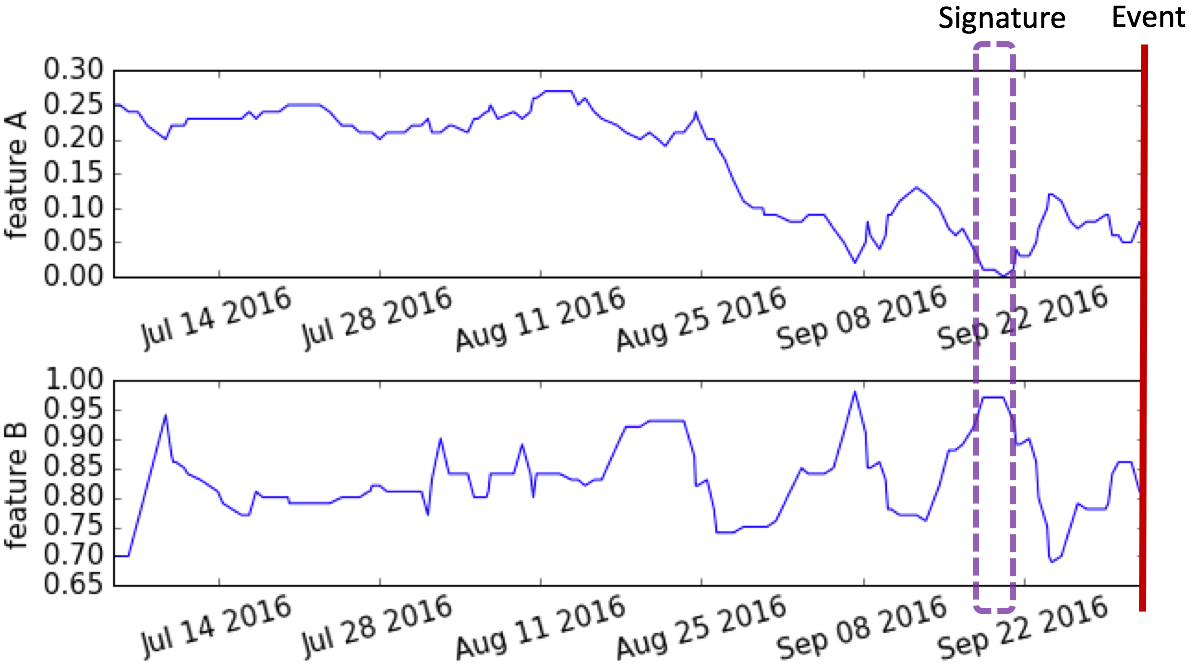
\includegraphics[width=3.1in]{pics/Motivation_1} \label{fig:MAMT:motivation:01}}
\subfigure[Event 2]{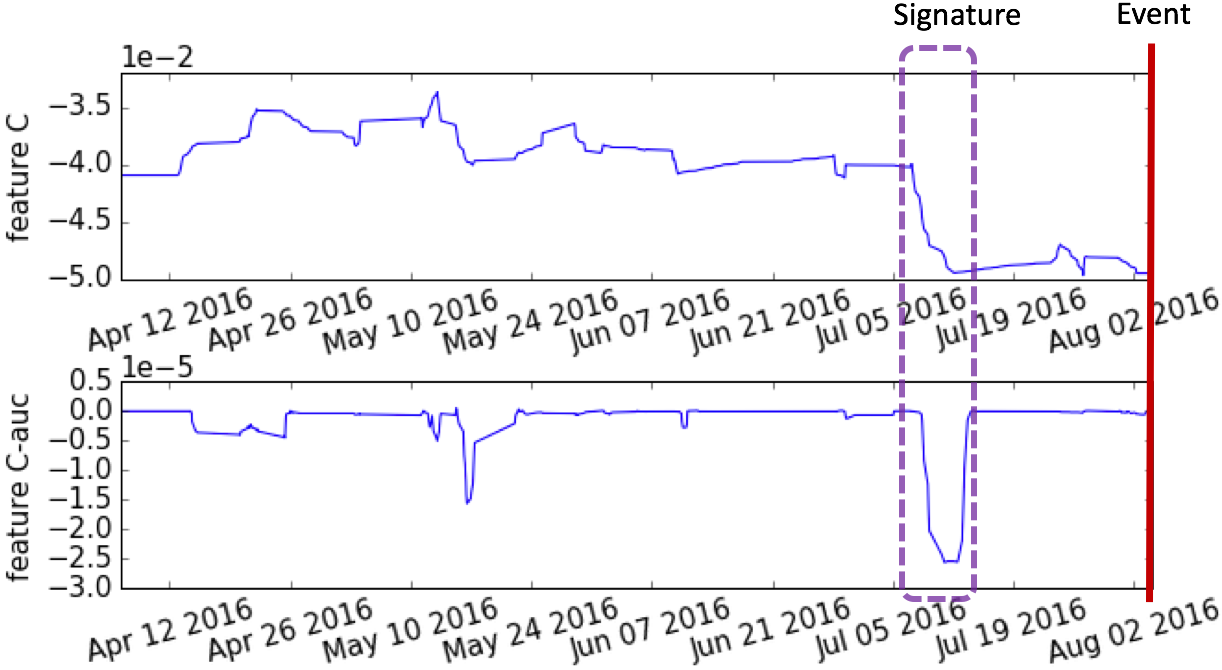
\includegraphics[width=3.1in]{pics/Motivation_2} \label{fig:MAMT:motivation:02}}
\caption{Two examples of fault signatures with lag to final failures (events). In Figure~\ref{fig:MAMT:motivation:01} the signature appears $15$ days before the failure, with small value on feature A and large value on feature B. While in Figure~\ref{fig:MAMT:motivation:02} the signature appears almost one month before the failure, where there is a level-shift on feature C that can be capture by auto-correlation (auc).}
\label{fig:MAMT:motivation}
\end{figure}

\begin{figure*}[tb]
\centering
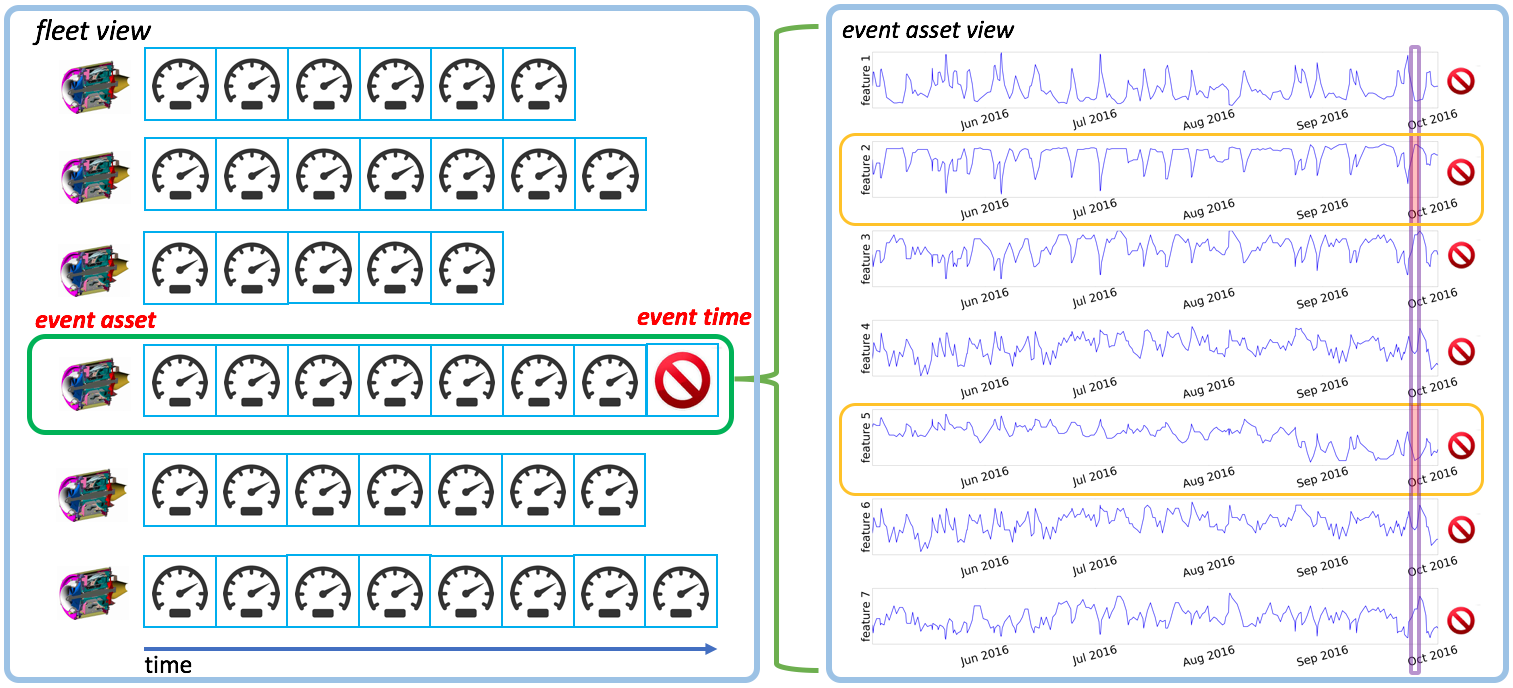
\includegraphics[width=5in]{pics/multi-view_structure}
\caption{Illustration of Multi-view Failure Analysis on Multivariate Time-series Data. Given the event asset and event time on the fleet level data, our model can provide the fault signature (marked by red shadow) on the feature level (rounded by yellow box) and timestamp level (rounded by purple box). }
\label{fig:MAMT:structure}
\end{figure*}

It can be easily imagined that, if we natively label the samples right before failure as ``1" and perform classic supervised machine learning algorithm \footnote{In a classic supervised setting, the event samples are considered as positive and usually labeled as ``1", while the other are considered as normal and labeled as ``0".}, we are not able to find such fault signature. The key difference of the problem, compared to the popular definition of supervised problems, is that \textbf{our label ``1"s are uncertain and even most of them could be wrong}. For example in Figure~\ref{fig:MAMT:motivation:01}, without any prior knowledge if we label all samples $30$ days before the final failure as ``1", the classic feature selection like random forest, lasso-based or mutual-information based methods will be easily failed, since only $10\%$ of ``1" are correct and the rest should be treated as $0$ (normal class). To handle this kind of problem, this paper proposes a Multi-view Failure Analysis on 
Multivariate Time-series Data (MAMT) which overcomes the limitations of classic supervised algorithms on such problem.  Our contributions are as follows:
\begin{enumerate}[(1)]
\item We proposed a novel fleet analytics model that aims to select key features that relate to the failure on multivariate time-series data, which can effectively support the root cause analysis.
\item Our proposed model, compared with the existing supervised methods, automatically detect the time of signature by filtering the ``wrong labels". 
\item Our proposed model, compared with the existing methods,
    achieves a similar or even lower time and space computational complexity, but a more desired effectiveness.
\end{enumerate}



Figure~\ref{fig:MAMT:structure} illustrates that such multi-view analytics is unique and different from the existing works on any supervised feature selection or instance selection for multivariate temporal data. The left side shows the data on the fleet-level view and the event asset and event time is already known. The right side shows the multivariate time series for the event asset, and the fault signature on the feature level (rounded by yellow box) and timestamp level (rounded by purple box) are unknown. Without any more prior knowledge (other than the event asset and event time), our model can provide the fault signature (marked by red shadow) on multi-view level.   


%Capabilities of this algorithm: 
%Output corresponding classifier/detector to detect the targeted failure events on the fleet level.
%Automatically detect the most relevant feature patterns among all events that support root cause analytics. 
%Automatically adapt/detect different lead time for each event.   

\section{Problem Definition}
\label{sec:MAMT:prb_def}

In this section, we will mathematically define our problem setting.  
We start off by formally defining our notation. 
For a matrix $Z \in \mathbb{R}^{m \times n}$, $Z^\top$ denotes its transpose, and $Z^{-1}$ denotes its (pseudo)inverse. 
We also use entry-wise norms denoted by $\|Z\|_p$, where $p=2$ gives (Frobenius norm) $\| Z \|_F^2 = \sum_{ij}z^2_{i,j} = \mathrm{tr}(Z^\top Z)$, and $p=(2,1)$ gives the $\ell_{2,1}$ norm $\|Z\|_{2,1} =  \sum_{i=1}^{m}\|z^2_{i,:}\|$ where $z_{i,:}$ denotes the $i$th row of $Z$. 
For a vector $(w_1,...,w_m) \in \mathbb{R}^{m\times1}$, $\mathrm{diag}(w_1,...,w_m) \in \mathbb{R}^{m \times m}$ denotes a diagonal matrix with $w_1,...,w_m$ as its diagonal entries. Let $\mathbb{I}_m$ denote an identity matrix of dimension $m \times m$. 


Let $\textbf{X} = [x_1, x_2, ..., x_n] \in \mathbb{R}^{m \times n}$ where $x_i$ represents a sample ($m \times 1$ vector) at a certain timestamp in a time series feature space, and $\textbf{f} = [f_1, f_2, ..., f_m]$ be the set of features.  On a fleet level analytics, $\textbf{X}$ may involve samples from a few assets. And the feature set may not only include the raw sensors output, but also the transformed time series features, which could be created by sliding-window-based methods like mean, variance and auto-correlation. We will further discuss the ways of time series feature transformation in Section \ref{sec:MAMT:experiment}. 

Now consider we have one event asset and the event time is already known. With certain domain knowledge, we can confidently assume that the fault appears no earlier than $a$ timestamp samples right before the failure.  Without loss of generality, let $\textbf{X}_\textbf{a} = [x_1, x_2, ..., x_{a}] \in \mathbb{R}^{m \times a}$ represent the $a$ timestamp samples right before the failure,  and $\textbf{X}_\textbf{b} = [x_{a+1}, x_{a+2}, ..., x_{a+b}] \in \mathbb{R}^{m \times b}$ represent all the other samples we consider as normal and irrelevant to the failure, and usually $b \gg a$. We denote $\textbf{X} = [\textbf{X}_\textbf{a}, \textbf{X}_\textbf{b}] \in \mathbb{R}^{m \times n}$ where $n = a+b$. The output we expect is a feature score vector $\textbf{W} \in \mathbb{R}^{m \times 1}$, and a instance score vector $\textbf{Y}_\textbf{a} \in \mathbb{R}^{1 \times a}$, where each element represents the contribution of the feature/instance to the fault. The larger the value is, the more relevant the feature/instance is to the fault.   





\section{Algorithm}
\label{sec:MAMT:alg}

The key difference of this problem, compared against the popular definition of supervised problems, is that while our label ``0"s (or most of them, if not all) are reliable since we know there is not similar failure happened at those time or assets, our label ``1"s are uncertain and even most of them could be wrong. In this section we introduce our framework to solve this problem, which consists of supervised feature selection and dynamic and directional label propagation. 

\subsection{Supervised Feature Selection}
\label{sec:MAMT:alg:fea_sel} 
Intuitively, the requirement of failure signature analytics makes it closely connected to supervised feature selection. Thereby we first introduce a representative feature selection method based on  $\ell_{2,1}$ norm regularization ~\cite{liu2009multi} as our baseline feature selection algorithm. 

\begin{align}
\label{eq1:MAMT:l21}
& \min_{W} \| W^\top X - Y\|_F^2 + \alpha\|W\|_{2,1}, 
\end{align}
where $X \in \mathbb{R}^{m \times n}$ is the input dataset with $n$ samples and $m$ features, and $Y \in \mathbb{R}^{1 \times n}$ is the label vector in a binary classes setting with ``1" means the corresponding sample is considered as interesting and ``0" means it is normal sample. The final output $W \in \mathbb{R}^{m \times 1}$ gives a feature weighting vector represents the importance of each feature to the classification. 

The problem in Eq.\ref{eq1:MAMT:l21} can be interpreted as a generalized $\ell_{2,1}$ norm regularization problem~\cite{liu2009multi}, where the first term is a smooth convex loss function, and the second term controls the capacity of $W$ and also ensures that $W$ is sparse in rows, with the parameter $\alpha$ controlling the sparsity of $W$.   

\subsection{Dynamic and Directional Label Propagation}
\label{sec:MAMT:alg:lbl_ppg} 
As we mentioned earlier, what makes this problem unique to the popular feature selection, is that the label vector $Y$  is not able to be relied on. In some application cases it could be over $90\%$ mislabeled. Given such serious noisy labeling situation, the popular feature selection, and even the existing work on handling noisy labels ~\cite{tang2013coselect, frenay2014estimating} will easily fail since their assumption is only a small portion of labels are wrong. 

Here we introduce a Dynamic and Directional Label Propagation which can iteratively filter out wrong labels while maintaining those right ones. We start off by briefly describing the classic Label Propagation technique~\cite{wang2008graph, nie2010general}.  Consider a regularization framework on graph, the cost function associated with label propagation of $Y$ is defined as
\begin{align}
\label{eq1:MAMT:lbl_ppg}
& \min_{Y}  \sum_{i,j=1}^n \tilde{A}_{ij}\|Y_i-Y_j\|_F^2+\mu\sum_{i=1}^n\|Y_i-E_i\|^2,
\end{align}
where $Y \in \mathbb{R}^{1 \times n}$ is the label vector in a binary classes setting with ``1" means the corresponding sample is considered as interesting and ``0" means it is normal sample, $E \in \mathbb{R}^{1 \times n}$ is the label initialization, and $\tilde{A} \in \mathbb{R}^{n \times n}$  is a normalized affinity matrix.  The problem in Eq.\ref{eq1:MAMT:lbl_ppg} can be interpreted as a trade-off optimization problem, where the first term is a global smoothness meaning that two close samples should share the same labels, and the second term is a local fitness meaning that the final label should not be dramatically different from the initial seed, with parameter $\mu$ controlling the trade-off.  Label Propagation has strong connection with random walk, in the way that the label propagate out with the process of random walk~\cite{nie2010general}, which built upon a stable transition probability among samples. Figure~\ref{fig:MAMT:lbl_ppg:cls} shows the illustration of classic label propagation in a binary setting. We can see that given the initial label seed and a well constructed graph, the final label shows good classification result. 

\begin{figure}[htb]
\centering
\subfigure[classic label propagation]{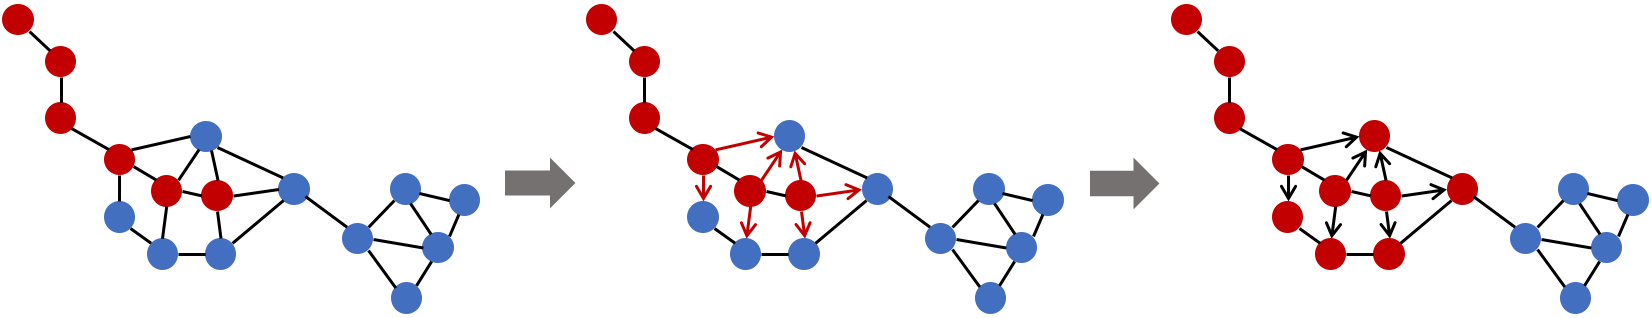
\includegraphics[width=3.3in]{pics/classic_label_propagation} \label{fig:MAMT:lbl_ppg:cls}}
\subfigure[Directional Label Propagation]{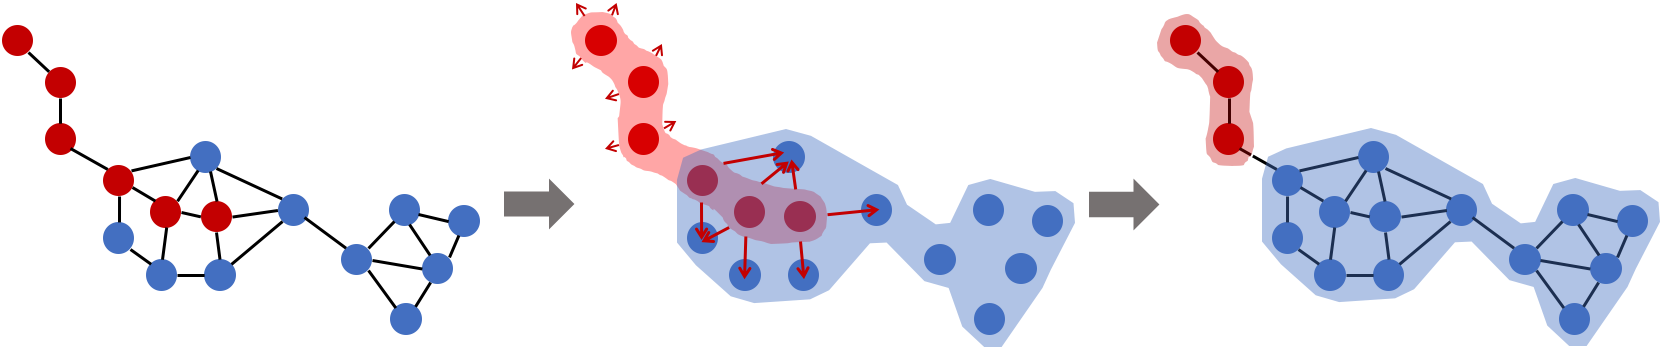
\includegraphics[width=3.3in]{pics/directional_label_propagation} \label{fig:MAMT:lbl_ppg:drc}}
\caption{Illustration of classic and our proposed label propagation. Red indicates the samples labeled as ``1" and blue as the ``0". }
\label{fig:MAMT:lbl_ppg}
\end{figure}

However, we have a different purpose in our problem setting:  \textbf{our goal is more on filtering out the wrong ``1" rather than expanding the right ``1"}.  Therefore, instead of constructing an omnidirectional random walk,  we model the propagation through a directional random walk as shown in Figure~\ref{fig:MAMT:lbl_ppg:drc}. Given the whole dataset as $\textbf{X} = [\textbf{X}_\textbf{a}, \textbf{X}_\textbf{b}] \in \mathbb{R}^{m \times n}$ with $m$ features and $n$ samples, and $\textbf{X}_\textbf{a} \in \mathbb{R}^{m \times a}$ is initially labeled as ``1" while $\textbf{X}_\textbf{b} \in \mathbb{R}^{m \times b}$ as ``0", we can construct a similarity matrix $A \in \mathbb{R}^{n \times n}$. We split matrix $A$ into $4$ blocks
\begin{align}            
\label{eq1:MAMT:A_block:01}
A = 
\begin{bmatrix}
A_{aa}&A_{ab}\\
A_{ba}&A_{bb}
\end{bmatrix},
\end{align}
where $A_{aa}$ describes the transition within $\textbf{X}_\textbf{a}$ and $A_{ab}$ describes the transition from $\textbf{X}_\textbf{a}$ to $\textbf{X}_\textbf{b}$ and so forth. 

In our problem setting, we assume that the samples in $\textbf{X}_\textbf{a}$ that labeled incorrectly in the initial seed are closed to (partial of) $\textbf{X}_\textbf{b}$ on all the feature subspace, and only those labeled correctly as ``1" are separable from $\textbf{X}_\textbf{b}$ in certain feature subspace. Therefore in a specifically designed label propagation, we hope the wrong ``1" is propagated out to its ``0" neighborhood and the right ``1" can be maintained. Detailedly speaking, we allow the ``1" labels propagate from $\textbf{X}_\textbf{a}$ to $\textbf{X}_\textbf{b}$ only, but not propagate back to $\textbf{X}_\textbf{a}$. Also we do not pay attention to the propagation within $\textbf{X}_\textbf{b}$ since no relevant event happened here and all these samples are assumed to be normal. Furthermore, we only allow self-loop exist in $\textbf{X}_\textbf{a}$ so the right ``1" can be conserved even there is high density in $\textbf{X}_\textbf{a}$. Therefore matrix $A$ is redefined as 
\begin{align}            
\label{eq1:MAMT:A_block:02}
A = 
\begin{bmatrix}
\mathrm{diag}(A_{aa})&A_{ab}\\
\textbf{0}_{ba}&\textbf{0}_{bb}
\end{bmatrix},
\end{align}  
where the lower part of $A$ are set to be $\textbf{0}$ matrix. Figure~\ref{fig:MAMT:lbl_ppg:drc} shows the illustration of our proposed Directional Label Propagation. We can see that given directional control, the wrong labels are ``flipped" and only the right ones conserved. 

\subsection{Our Proposed Framework}
\label{sec:MAMT:alg:framework} 
With our solutions to both feature side and label side, we are ready to introduce the Multi-view Failure Analysis on Multivariate Time-series Data (MAMT) framework. Considering both selecting the key feature (Eq.\ref{eq1:MAMT:l21}) and rectifying the labels (Eq.\ref{eq1:MAMT:lbl_ppg}), MAMT is to solve the following optimization 
\begin{align*}
\label{eq1:MAMT:mamt}
\mathcal{M}(W, \hat{Y}) &= \min_{W, \hat{Y}}  \| W^\top XB - \hat{Y}B\|_F^2 + \alpha\|W\|_{2,1} + \gamma\|\hat{Y}\|_{2,1}\\&+ \delta\bigg[\sum_{i,j=1}^n \tilde{A}_{ij}\|\hat{Y}_i-\hat{Y}_j\|_F^2+\mu\sum_{i=1}^n\|\hat{Y}_i-E_i\|^2\bigg],
\end{align*}
where $\hat{Y} = Y \circ E$ is the Hadamard product of $Y$ and $E$, while 
$E = [\textbf{1}_a, \textbf{0}_b] \in \mathbb{R}^{1 \times n}$ is the initial labels with $\textbf{1}_a = [1,1,...,1] \in \mathbb{R}^{1 \times a}$ corresponds to $\textbf{X}_\textbf{a}$ and $\textbf{0}_b = [0,0,...,0] \in \mathbb{R}^{1 \times b}$ corresponds to $\textbf{X}_\textbf{b}$, and $B = \mathrm{diag}([\beta\textbf{1}_a, \textbf{1}_b])$ is the sample weights in a diagonal format. The reason of bringing $\hat{Y}$ is because we want to ``compress" the label of $\textbf{X}_\textbf{b}$ all the time, and the reason of bringing $B$ is to handle the imbalance problem between $\textbf{X}_\textbf{a}$ and $\textbf{X}_\textbf{b}$. Please note that we also bring in a  $\ell_{2,1}$ norm regularization on $\hat{Y}$ to emphasize its scarcity in the final solution. In Section \ref{sec:MAMT:alg:proof_early} we will verify that the $\mathcal{M}(W, \hat{Y})$ is joinly convex with $W$ and $\hat{Y}$. 
 
It is difficult to optimize $W$ and $\hat{Y}$ simultaneously. Therefore we adopt an alternating optimization to solve this problem, which works well for a number of practical optimization problems\cite{feng2012adaptive, tang2013coselect}. 

\smallskip
\noindent\textbf{Given $\hat{Y}$, optimize $W$.}

\smallskip
\noindent\textbf{Given $W$, optimize $\hat{Y}$.}

\subsection{\color{red}{Proof and Early Stopping} }
\label{sec:MAMT:alg:proof_early} 

\subsection{Whole algorithm}
\label{sec:MAMT:alg:alg} 
%\section{Proof}
If any proof is needed.
\label{sec:MAMT:proof}

\section{Complexity Analysis and Lighter Implementation}

\label{sec:MAMT:cmplexity}

\section{Related Work and Discussion}

\label{sec:MAMT:discussion}

\begin{enumerate}[(1)]
\item L.
\item Manifold on Xa. 
\item multi-events.
\end{enumerate}

\section{Experiment}

\label{sec:MAMT:experiment}

\section{Conclusion}

\label{sec:MAMT:conclusion}



\bibliography{ref}
\bibliographystyle{plain}





% that's all folks
\end{document}


